%--------------------------------------------------------------
% tesi.tex 
%--------------------------------------------------------------
% Corso di Laurea in Informatica 
% http://if.dsi.unifi.it/
% @Facolt\`a di Scienze Matematiche, Fisiche e Naturali
% @Universit\`a degli Studi di Firenze
%--------------------------------------------------------------
% - template for the main file of Informatica@Unifi Thesis 
% - based on Classic Thesis Style Copyright (C) 2008 
%   Andr\'e Miede http://www.miede.de   
%--------------------------------------------------------------

\documentclass[twoside,openright,titlepage,fleqn,
,	headinclude,12pt,a4paper,BCOR5mm,footinclude,table]{scrbook}
%--------------------------------------------------------------
\newcommand{\myItalianTitle}{Sistema client-server per la ricerca del cammino minimo in un grafo con topologia a griglia\xspace}
\newcommand{\myEnglishTitle}{\xspace}
% use the right myDegree option
\newcommand{\myDegree}{Corso di Laurea Magistrale in Informatica\xspace}
%\newcommand{\myDegree}{
	%Corso di Laurea Specialistica in Scienze e Tecnologie 
	%dell'Informazione\xspace}
\newcommand{\myName}{Tommaso Puccetti, Alex Foglia, Francesco Secci\xspace}
\newcommand{\myProf}{\xspace}
\newcommand{\myOtherProf}{Nome Cognome\xspace}
\newcommand{\mySupervisor}{Nome Cognome\xspace}
\newcommand{\myFaculty}{
	Scuola di Scienze Matematiche, Fisiche e Naturali\xspace}
\newcommand{\myUni}{\protect{
	Universit\`a degli Studi di Firenze}\xspace}
\newcommand{\myLocation}{Firenze\xspace}
\newcommand{\myTime}{Anno Accademico 2017-2018\xspace}
\newcommand{\myVersion}{Version 0.1\xspace}
%--------------------------------------------------------------

\usepackage[italian]{babel}
\usepackage[latin1]{inputenc} 
\usepackage[T1]{fontenc} 
\usepackage[square,numbers]{natbib} 
\usepackage[fleqn]{amsmath}  
\usepackage{ellipsis}
\usepackage{listings}
\usepackage{subfig}
\usepackage{caption}
\usepackage{appendix}
\usepackage{siunitx}
\usepackage{url}

%--------------------------------------------------------------
\usepackage{dia-classicthesis-ldpkg}
%--------------------------------------------------------------


%
% Options for classicthesis.sty:
% tocaligned eulerchapternumbers drafting linedheaders 
% listsseparated subfig nochapters beramono eulermath parts 
% minionpro pdfspacing
\usepackage[eulerchapternumbers,linedheaders,subfig,beramono,eulermath,
parts]{classicthesis}
%--------------------------------------------------------------
\newlength{\abcd} % for ab..z string length calculation
% how all the floats will be aligned
\newcommand{\myfloatalign}{\centering} 
\setlength{\extrarowheight}{3pt} % increase table row height
\captionsetup{format=hang,font=small}
%--------------------------------------------------------------
% Layout setting
%--------------------------------------------------------------
\usepackage{geometry}
\geometry{
	a4paper,
	ignoremp,
	bindingoffset = 1cm, 
	textwidth     = 13.5cm,
	textheight    = 21.5cm,
	lmargin       = 3.5cm, % left margin
	tmargin       = 4cm    % top margin 
}




%%
%% Julia definition (c) 2014 Jubobs
%%
\lstdefinelanguage{Julia}%
  {morekeywords={abstract,break,case,catch,const,continue,do,else,elseif,%
      end,export,false,for,function,immutable,import,importall,if,in,%
      macro,module,otherwise,quote,return,switch,true,try,type,typealias,%
      using,while},%
   sensitive=true,%
   alsoother={},%
   morecomment=[l]\#,%
   morecomment=[n]{\#=}{=\#},%
   morestring=[s]{"}{"},%
   morestring=[m]{'}{'},%
}[keywords,comments,strings]%

\lstset{%
    language         = Julia,
    basicstyle       = \ttfamily,
    keywordstyle     = \bfseries\color{blue},
    stringstyle      = \color{magenta},
    commentstyle     = \color{ForestGreen},
    showstringspaces = false,
}
%%%

\usepackage{tikz}
\usetikzlibrary{arrows}
\usetikzlibrary{positioning}
\tikzset{main node/.style={circle,fill=blue!20,draw,minimum size=1cm,inner sep=0pt},
            }



%--------------------------------------------------------------
\begin{document}
\frenchspacing
\raggedbottom
\pagenumbering{roman}
\pagestyle{plain}
%--------------------------------------------------------------
% Frontmatter
%--------------------------------------------------------------




\pagestyle{scrheadings}
%--------------------------------------------------------------
% Mainmatter
%--------------------------------------------------------------
\pagenumbering{arabic}
% use \cleardoublepage here to avoid problems with pdfbookmark
%\include{intro} % use \myChapter command instead of \chapter
%\cleardoublepage\myPart{Part I}
%\include{chapter01}
%\cleardoublepage\myPart{Part II}
%\include{chapter02}
%\include{chapter03}
%--------------------------------------------------------------
% titlepage.tex (use thesis.tex as main file)
%--------------------------------------------------------------
\begin{titlepage}
	\begin{center}
   	\large
      \hfill
      \vfill
      \begingroup
     
        Advanced Techniques and Tools for Software Development
           
      \endgroup 
      \vfill 
      \begingroup
      	\color{Maroon}\spacedallcaps{\myItalianTitle} \\ $\ $\\
      	\spacedallcaps{\myEnglishTitle} \\ 	
	\bigskip
      \endgroup
      \spacedlowsmallcaps{\myName}
      \vfill 
      \vfill
    
      \vfill
      \vfill
      \myTime
      \vfill                      
	\end{center}        
\end{titlepage}   
%--------------------------------------------------------------
% back titlepage
%--------------------------------------------------------------
   \newpage
	\thispagestyle{empty}
	\hfill
	\vfill
	\noindent\myName: 
	\textit{\myItalianTitle,} 
	\myDegree, \textcopyright\ \myTime
%--------------------------------------------------------------
% back titlepage end
%--------------------------------------------------------------
\tableofcontents
\listoftables
\listoffigures
\chapter{Sistema implementato}
\section{Panoramica ad alto livello}
Il sistema che abbiamo implementato \`e una \emph{web-app} la cui funzione \`e quella di ricercare il cammino minimo in un grafo con topologia a griglia, dati due particolari nodi: uno di partenza e uno di arrivo.\\*
Una \emph{griglia} \`e rappresentata attraverso una matrice $A \in \mathbb{N}^{n x n}$ siffatta:
\[ A=[a_{i,j}] \]
Dove $a_{i,j}>0 \iff \exists $ un nodo nella riga i e colonna j della griglia rappresentata da $A$ e $n$ \`e il numero massimo di righe e colonne ammesso per la griglia che A rappresenta.\\*
Occorre precisare che in questa particolare topologia di grafo, ogni nodo $i,j$ pu\`o avere al pi\`u 4 vicini:
\begin{itemize}
	\item $i+1,j$
	\item $i-1,j$
	\item $i,j+1$
	\item $i,j-1$
\end{itemize} 
Pertanto il cammino minimo potr\`a attraversare archi solo in direzione orizzontale o verticale.\newpage
A titolo di esempio, si consideri la matrice in tabella 1.
\begin{table}[]
	\centering
	\caption{Matrice A}
	\label{my-label}
	\begin{tabular}{|l|l|l|l|l|}
		\hline
		1 & 0 & 1 & 0 & 0 \\ \hline
		1 & 1 & 1 & 0 & 0 \\ \hline
		1 & 0 & 0 & 0 & 1 \\ \hline
		1 & 1 & 1 & 1 & 1 \\ \hline
		0 & 0 & 0 & 0 & 1 \\ \hline
	\end{tabular}
\end{table}
Supponiamo di voler cercare il camminimo minimo che parta dal nodo $0,0$ e che termini al nodo $4,4$ (nella fattispecie, esso \`e unico).
Si ottiene il risultato esposto in tabella 2.
\begin{table}[]
	\centering
	\caption{Cammino minimo relativo ad A}
	\label{my-label}
	\begin{tabular}{|l|l|l|l|l|}
		\hline
		\cellcolor[HTML]{68CBD0}1 & 0 & 1 & 0 & 0                         \\ \hline
		\cellcolor[HTML]{68CBD0}1 & 1 & 1 & 0 & 0                         \\ \hline
		\cellcolor[HTML]{68CBD0}1 & 0 & 0 & 0 & 1                         \\ \hline
		\rowcolor[HTML]{68CBD0} 
		1                         & 1 & 1 & 1 & 1                         \\ \hline
		0                         & 0 & 0 & 0 & \cellcolor[HTML]{68CBD0}1 \\ \hline
	\end{tabular}
\end{table}
\newpage
L'implementazione del suddetto sistema si articola in due componenti:
\begin{enumerate}
	\item Server
	\item Client
\end{enumerate}
Il Server, realizzato attraverso l'utilizzo del framework \emph{Spring Boot}, gestisce un database MongoDB contenente le matrici che rappresentano particolari griglie.\\*
Il Server deve poter essere in grado di gestire tre tipi di richieste pervenibili attraverso la sua interfaccia \emph{REST}: recuperare tutte le griglie salvate nel database, recuperarne una in particolare, oppure trovare un eventuale cammino minimo in una particolare griglia.\\*
Per quanto riguarda le operazioni \emph{CRUD} sul database, queste sono realizzate mediante un \emph{Web Controller} protetto da username e password. Occorre infine precisare che il server non \`e consapevole di colloquiare con una particolare istanza di un client, ci\`o comporta che le richieste vengano ugualmente servite sia nel caso in cui il client sia un normale browser, oppure il Client java che abbiamo realizzato.\\*
Il Client da noi implementato \`e un' applicazione Java che utilizza la libreria \emph{Swing} per fornire all'utente un'interfaccia grafica \emph{user-friendly}. Il Client \'e capace di eseguire le tre possibili richieste \emph{HTTP} inoltrabili all'interfaccia \emph{REST} del Server.
\begin{figure}[th]
	\centering
	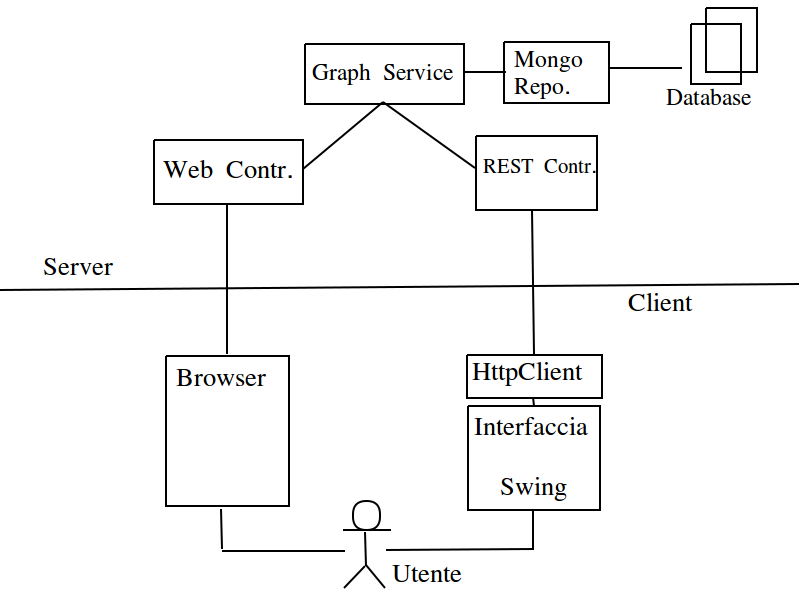
\includegraphics[width=0.7\linewidth]{Images/app-scheme}
	\caption[Schema UML-Like]{Schema che mostra il funzionamento del sistema implementato cos\`i come visto dall'utente}
	\label{fig:app-scheme}
\end{figure}


\chapter{Tecniche e framework utilizzati}
\section{Code versioning}
Per tenere traccia della storia dei codici di Server e Client abbiamo utilizzato il software \emph{git} creando una repository locale connessa a una repository remota su \emph{github}. La repository remota utilizzata \`e disponibile per la consultazione al seguente URL:
\begin{itemize}
	\item \url{https://github.com/alexfoglia1/attsw-server}
\end{itemize}
L'utilizzo di \emph{git} si \`e rivelato particolarmente utile per il lavoro in gruppo, grazie al meccanismo delle \emph{pull requests}. Il workflow che abbiamo seguito prevedeva di aprire un ramo ogni qualvolta un membro del gruppo volesse implementare una particolare \emph{feature} all'interno dei software. Abbiamo dunque realizzato sul master tutte le interfacce di cui gli applicativi faranno uso e creato un ramo per ogni loro singola implementazione. Quando una particolare implementazione veniva terminata, allora procedevamo al \emph{merge} del ramo sul master risolvendo gli eventuali conflitti generati, mediante l'interfaccia di \emph{github}.\\*
Non abbiamo sollevato alcuna \emph{issue} perch\`e abbiamo lavorato per la maggior parte del tempo nel medesimo luogo fisico.\\*
\emph{Git} \`e stato utilizzato sia da terminale, che tramite il plugin per eclipse \emph{e-git} che ci ha semplificato alcune operazioni.\\*
\section{Dependencies and build tool}
Per gestire le dipendenze e realizzare la build del codice, abbiamo utilizzato il software \emph{Apache Maven}, in particolare ne abbiamo utilizzato la sua integrazione nativa in eclipse.\\*
Dal momento che occorre fornire evidenze su metriche quali \emph{code coverage} e qualit\`a del codice abbiamo realizzato i seguenti profili Maven all'interno del POM con lo scopo di eseguire differenti processi di build in relazione ai particolari plugin che era necessario legare a ciascuna fase del ciclo di vita di Maven.
\begin{lstlisting}
clean verify -Pjacoco coveralls:report
clean verify -Pjacoco sonar:sonar
clean verify -Pfailsafe
\end{lstlisting}
Il profilo jacoco serve a generare i report sugli unit test e ad inviarli rispettivamente ai server di \emph{Coveralls} e di \emph{SonarQube} (\emph{SonarCloud}); mentre il profilo failsafe esegue sia gli unit test che gli integration test ed \`e proprio quest'ultima build quella che effettuiamo anche in locale. Dal momento che il codice del progetto si articola in 3 moduli (Client, Server, End2End), il comando di build viene eseguito nella directory del parent pom che accomuna i sopracitati moduli.
\section{Continuos integration}
Le repository elencate in 2.1 sono collegate al server di Continuos Integration \emph{Travis} attraverso il file \emph{.travis.yml}. Questo file rappresenta lo script che \emph{Travis} deve eseguire sulle macchine remote al fine di ricreare un ambiente in cui \`e possibile lanciare le stesse build che effettuiamo anche in locale. Per ricreare l'ambiente \emph{Travis} viene configurato in modo tale da usare il servizio Docker, ma \`e solo durante la build che viene lanciato il container Docker di MongoDB, in quanto il profilo failsafe, che deve eseguire gli integration test, \`e stato appositamente configurato per lanciare il container Docker legandone il relativo plugin alla fase \emph{pre-integration-test}. Dal momento che ciascuna build viene eseguita usando i profili jacoco e failsafe definiti nel POM, questa genera i report su \emph{Coveralls} e \emph{SonarCloud} sia nel caso in cui la build venga fatta in locale che sui server di \emph{Travis}. 
\section{Frameworks}
\subsection{Spring Boot}
Nel capitolo 1 si menziona Spring Boot quale framework utilizzato per realizzare il Server. Spring Boot \`e un particolare framework che facilita il programmatore nella realizzazione di una \emph{web-app} evitando allo stesso di utilizzare direttamente le Servlet Java. Spring Boot offre inoltre una libreria che implementa il design pattern \emph{Depencency Injection}, reso necessario dal meccanismo di \emph{Inversion of Control} sottostante una qualsiasi web-app Java. La \emph{Dependency Injection} \`e necessaria poich\'e springboot esegue la web-app all'interno di un web container il quale si trova a sua volta all'interno di un server, es. Tomcat. Infatti, proprio perch\'e la web-app viene lanciata all'interno di un web container, non possiamo avere il totale controllo sull'istanziazione degli oggetti a run-time.\\*Per questo motivo, Spring Boot, contestualmente al lancio dell'applicativo carica un particolare \emph{application-context} (contesto applicativo) il quale \`e l'insieme di tutti i bean che dovranno essere iniettati negli oggetti da essi dipendenti. Ogni bean iniettato \`e necessariamente un oggetto \emph{singleton}.
Le principali funzionalit\`a messe a disposizione da Spring Boot che abbiamo utilizzato sono le repository per i database e i controller per interfacciare la web-app verso l'esterno.\\*
Per realizzare il Server, al posto di eclipse, \`e stato utilizzato Spring Tool Suite, il quale ne rappresenta una versione modificata ad hoc.
\subsubsection{Scelta del database}
Spring Boot possiede librerie per gestire un ampio insieme di database; noi abbiamo scelto MongoDB in quanto funzionale alle necessit\`a dell'applicativo che intendevamo realizzare. MongoDB \`e un database NoSQL, questo implica che le entit\'a presenti al suo interno non devono rispettare alcun vincolo di integrit\'a realazionale, e questo ha particolarmente senso dal momento che nel database sono salvate istanze di griglie relazionalmente slegate l'una dall'altra. MongoDB \`e infine molto semplice da utilizzare ed integrare in una web-app.
\subsubsection{Template engine}
Spring Boot, per renderizzare le pagine html che un client pu\`o richiedere, utilizza l'engine \emph{Thymeleaf}.
\subsection{Framework di test}
Grazie alla sua facile integrazione con eclipse, gli unit test e gli integration test vengono eseguiti in locale utilizzando il framework \emph{Junit}. Per testare la corretta realizzazione dell'interfaccia utente di cui fa uso il Client abbiamo utilizzato il framework \emph{AssertJ}, che ci ha permesso di scrivere asserzioni sulle componenti grafiche realizzate.\\*
L'interfaccia del Client non \`e la sola interfaccia utente realizzata, infatti, come gi\`a specificato nel capitolo 1, il Server predispone un'interfaccia web dedicata alle operazioni CRUD sul database. Per testare questa interfaccia, che \`e necessariamente un'interfaccia HTML, abbiamo utilizzato il framework HtmlUnit. Per mockare le dipendenze delle classi durante il processo di test unitario abbiamo utilizzato il framework Mockito sia per il Client che per il Server.
\subsection{Http Client}
Per implementare le richieste HTTP del Client abbiamo scelto il framework \emph{Apache HttpClient} che mette a disposizione le classi necessarie per effettuare richieste HTTP su un particolare server (es. GET oppure POST) evitando di scrivere direttamente codice che usi le classiche Socket.
\subsection{GUI}
Il framework scelto per la realizzazione dell'interfaccia grafica \`e \emph{Swing}. Questo framework ci ha permesso di integrare Apache Http Client con una semplice interfaccia utente composta da una singola finestra (JFrame).
\subsection{End to end test}
Gli end to end test sono stati implementati usando Selenium per simulare la comunicazione browser-server; mentre Cucumber \`e il framework utilizzato per implementare gli end to end test secondo una tecnica BDD.
\chapter{Design e scelte implementative}

\section{Server}

Come gi\`a specificato nei precedenti capitoli, il Server deve esporre verso l'esterno due interfacce: l'interfaccia REST e l'interfaccia Web. Lo scopo della prima \`e quello di fornire un'interfaccia che consenta a un utente di poter:
\begin{itemize}
	\item Ricevere la lista di tutte le griglie presenti sul Server;
	\item Visualizzare una particolare griglia tra quelle disponibili;
	\item Richiedere un cammino minimo fra due nodi di una particolare griglia.
\end{itemize}
Per l'interfaccia Web, invece, \`e previsto che questa debba permettere all'utente di:
\begin{itemize}
	\item Inserire una griglia nel database;
	\item Visualizzare tutte le griglie salvate nel database;
	\item Eliminare una griglia dal database.
\end{itemize}
Entrambe le interfacce fanno uso di un'interfaccia interna all'applicazione: l'interfaccia \emph{IGridService}. Questa interfaccia ha il compito di fornire le operazioni necessarie per svolgere la funzione prevista dal sistema, ossia chi usa IGridService non vede i dettagli implementativi riguardanti come le operazioni di lettura e scrittura sul database vengono effettivamente realizzate. IGridService fornisce inoltre l'operazione di ricerca del cammino minimo, i cui dettagli verranno spiegati in seguito.
\subsection{Rappresentazione delle griglie}
Un oggetto griglia salvato nel database, viene visto dall'interfaccia IGridService come un'istanza della classe \emph{DatabaseGrid}. Questa classe \`e un wrapper di una matrice di interi, la quale rappresenta il grafo. La classe DatabaseGrid aggiunge inoltre informazioni su una griglia associando ad essa un intero (id) e un intero n che rappresenta il numero massimo di righe e colonne che devono essere lette dalla matrice wrappata per estrapolarne la griglia.\\*
Nonostante questa scelta sembra perdere di generalit\`a, in quanto considera solamente matrici quadrate, in realt\`a se volessimo rappresentare una griglia che non sia in generale quadrata, sarebbe sufficiente porre a 0 le righe o le colonne che non si vuole facciano parte del grafo.\\*
\subsection{REST Controller}
Il REST Controller che abbiamo realizzato \`e una classe, opportunamente annotata secondo la struttura di Spring Boot, che a run-time serve determinate richieste HTTP su tre particolari URL:
\begin{itemize}
	\item /api/ $\rightarrow$ restituisce al client una lista JSON di stringhe rappresentanti ciascun ID delle griglie salvate nel database.
	\item /api/grid$[i]$ $\rightarrow$ restituisce al client l'oggetto griglia avente id='i'  (serializzato come oggetto JSON);
	\item /api/path$[SOURCE]$TO$[SINK]$IN$[ID]$ $\rightarrow$ restituisce al client una lista JSON di stringhe rappresentanti i nodi che fanno parte del cammino minimo nel grafo con id='ID' partendo dal nodo 'SOURCE' e finendo nel nodo 'SINK'. Se il cammino non esiste, viene restituita una lista vuota.
\end{itemize}
La sintassi di un nodo, affinch\`e sia interpretabile dal server, deve rispettare la seguente espressione regolare:
$$
\texttt{[0-9]+\_[0-9]+}
$$
La prima cifra rappresenta l'indice di riga del nodo che si vuole considerare, mentre la seconda rappresenta l'indice di colonna.
\subsection{Web Controller}
Al Web Controller sono delegate le operazioni di aggiunta e rimozione di griglie all'interno del database. Tali operazioni sono concesse solo previa autenticazione con username e password. Per implementare il login abbiamo utilizzato la classe WebSecurityConfig, che comunica al framework di abilitare il sistema di login nativo di Spring Boot, escludendo da esso gli URL relativi all'interfaccia REST e permettendo l'accesso a qualsiasi altro URL solamente se identificati con nome utente "user" e password "password".\\*
Gli URL serviti dal Web Controller sono:
\begin{itemize}
	\item / $\rightarrow$ dalla root si accede a una pagina mediante la quale il client sceglie un particolare servizio del Web Controlller;

	
	\item /viewdb $\rightarrow$ viene renderizzata una pagina HTML nella quale sono riportate tutte le griglie presenti nel database;

	\item /addtable $\rightarrow$ viene renderizzata una pagina HTML che prevede l'immissione tramite un form di una griglia all'interno del database;
	
	\item /remtable $\rightarrow$ come addtable, ma il form richiede solo l'inserimento dell'id della griglia che si intende cancellare.
\end{itemize}
\newpage
	\begin{figure}[ht]
	\centering
	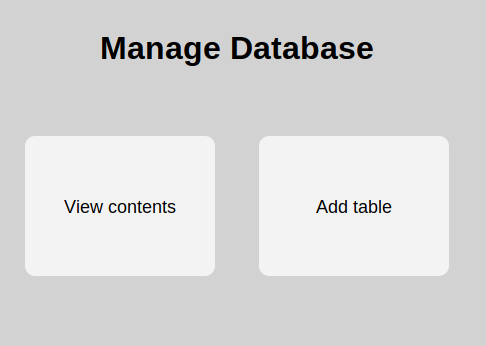
\includegraphics[width=0.7\linewidth]{Images/home}
	\caption{Home page della web-app}
	\label{fig:home}
\end{figure}
	\begin{figure}[ht]
	\centering
	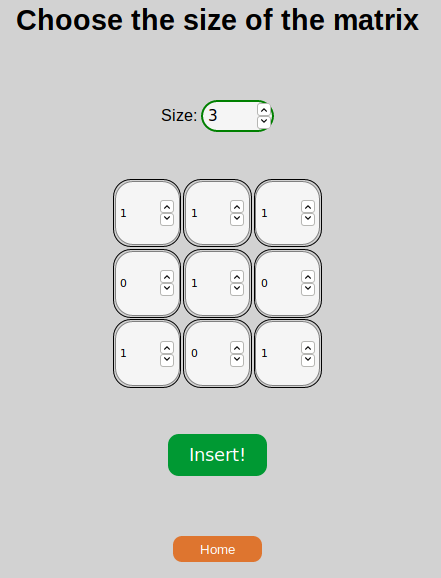
\includegraphics[width=0.7\linewidth]{Images/addtable}
	\caption{Form per l'inserimento di una nuova griglia}
	\label{fig:home}
\end{figure}
	\begin{figure}[ht]
	\centering
	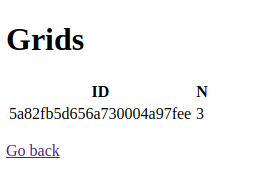
\includegraphics[width=0.7\linewidth]{Images/viewgrids}
	\caption{Lista delle griglie salvate nel database}
	\label{fig:home}
\end{figure}
	\begin{figure}[ht]
	\centering
	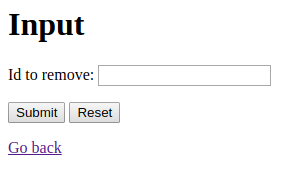
\includegraphics[width=0.7\linewidth]{Images/rem}
	\caption{Form per il cancellamento di una griglia}
	\label{fig:home}
\end{figure}
\newpage
\subsection{Algoritmo di ricerca del cammino minimo}
Per implementare la ricerca del cammino minimo in una griglia rappresentata dalla matrice A, la classe concreta che implementa IGridService (ConcreteGridService) opera nel modo seguente:
\begin{itemize}
	\item Per ogni nodo i,j di A tale che $A[i][j]>0$ aggiungi il nodo i,j a una lista \emph{nodes} di stringhe nella forma 	'$\texttt{i\_j}$';
	\item Per ogni nodo n di nodes:
	\begin{itemize}
		\item Controlla quali vicini ha n (controllando gli indici di riga e colonna come specificato nel capitolo 1)
		\item Se n ha un vicino n', allora aggiungi a una lista \emph{edges} di vettori di stringhe, l'arco $n\rightarrow n'$, dove ciascun arco e \`e un vettore di dimensione 2 tale per cui e$[0]=n$ ed e$[1]=n'$.
	\end{itemize}
\end{itemize}
A questo punto il grafo \`e completamente rappresentato dalla lista dei suoi nodi e dalla lista suoi archi, ed \`e possibile applicarvi il seguente algoritmo di visita per ricercare il cammino minimo tra due nodi source e sink.
\scriptsize
\begin{lstlisting}
Algoritmo cammino_minimo(source,sink):
	crea nodi_visitati;
	crea nodi_precedenti;
	crea lista_cammino_minimo;
	crea coda;
	Nodo corrente=source;
	coda.add(corrente);
	nodi_visitati.add(corrente,true);
	fintantoche(coda non vuota)
		corrente=coda.remove();
		se corrente==sink allora 
			esci;
		altrimenti
			per ogni nodo v vicino di current:
				se nodi_visitati non contiene v:
					coda.add(corrente);
					nodi_visitati(v,true);
					nodi_precedenti.add(v,corrente);
				fine se
			fine per
		fine se
	fine fintantoche
	se corrente != sink allora:
		restituisci lista vuota;
	altrimenti
		per Nodo n=sink, se n non nullo, n=nodi_precedenti.get(n):
			lista_cammino_minimo.add(n);
		fine per
		restituisci reverse(lista_cammino_minimo);
	fine se
fine algoritmo
\end{lstlisting}
\normalsize
\section{Client}
Il Client utilizza l'interfaccia IClient per colloquiare con l'interfaccia REST del Server. Questa classe utilizza al suo interno un'altra interfaccia, IRestServiceClient. Quest'ultima utilizza il framework Apache Http Client col fine di eseguire richieste HTTP sui particolari URL dell'interfaccia REST del Server che abbiamo realizzato. L'interfaccia IClient permette all'utente di:
\begin{itemize}
	\item ricevere la lista di tutte le griglie presenti sul database del Server;
	\item ricevere una particolare griglia;
	\item ricevere un particolare cammino minimo all'interno di una griglia.
\end{itemize}
Gli oggetti ricevuti sono stringhe JSON nel primo e nel terzo caso, mentre quando si riceve una particolare griglia, se ne riceve la serializzazione JSON. Una griglia serializzata tramite JSON viene poi caricata in memoria come un'istanza della classe GridFromServer; classe del tutto equivalente alla classe DatabaseGrid che abbiamo discusso in 3.1.1.
\subsection{Interfaccia utente}
L'applicazione mette a disposizione dell'utente la seguente interfaccia grafica per fare uso di un'implementazione concreta di IClient.
\begin{figure}[ht]
	\centering
	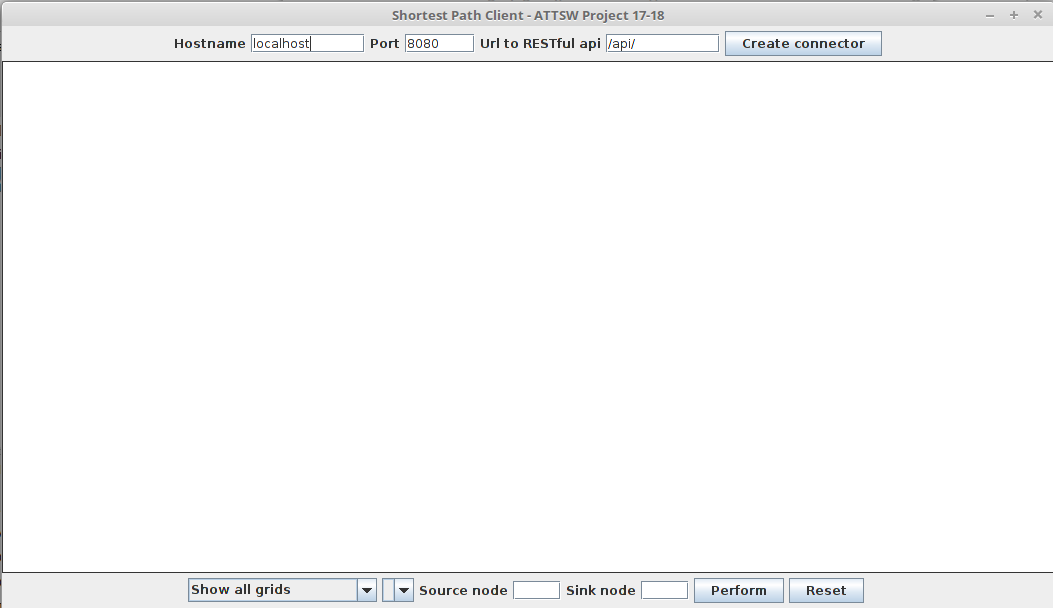
\includegraphics[width=0.7\linewidth]{Chapters/1}
	\caption[Interfaccia utente]{Interfaccia del Client all'avvio del sistema}
	\label{fig:1}
\end{figure}

\begin{figure}[ht]
	\centering
	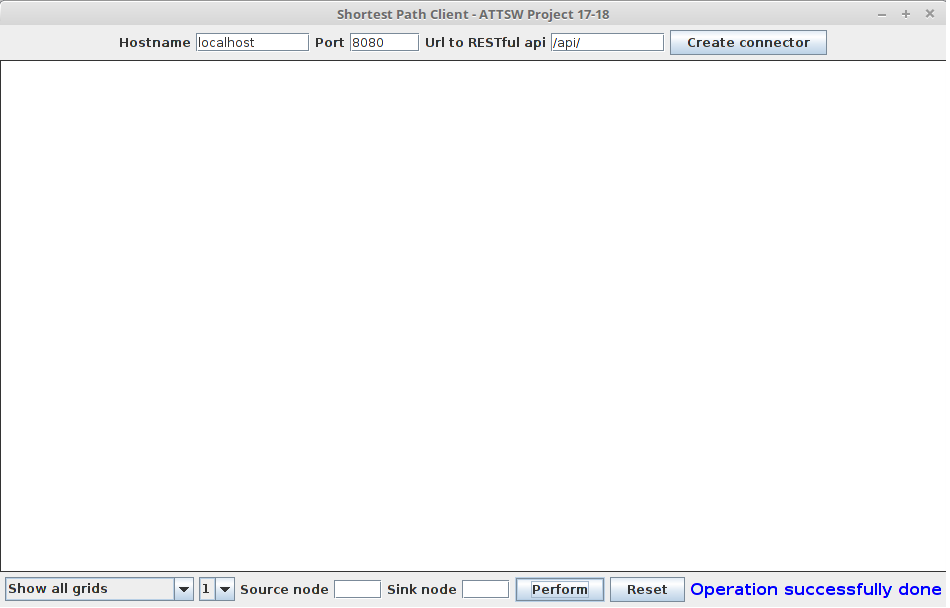
\includegraphics[width=0.7\linewidth]{Chapters/2}
	\caption[Interfaccia utente]{Richiedi tutte le griglie al Server}
	\label{fig:2}
\end{figure}

\begin{figure}[ht]
	\centering
	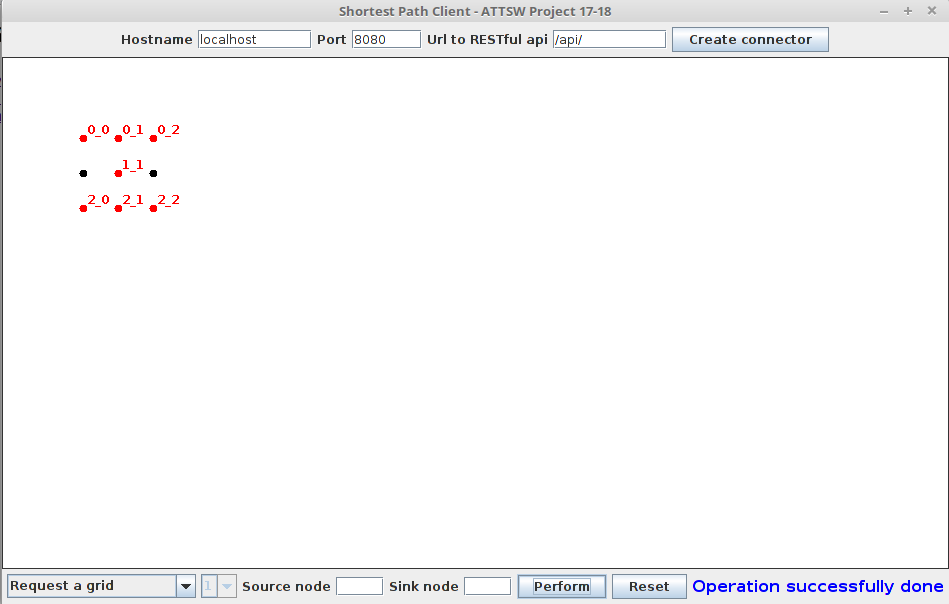
\includegraphics[width=0.7\linewidth]{Chapters/3}
	\caption[Interfaccia utente]{Richiedi griglia con id=1}
	\label{fig:3}
\end{figure}

\begin{figure}[ht]
	\centering
	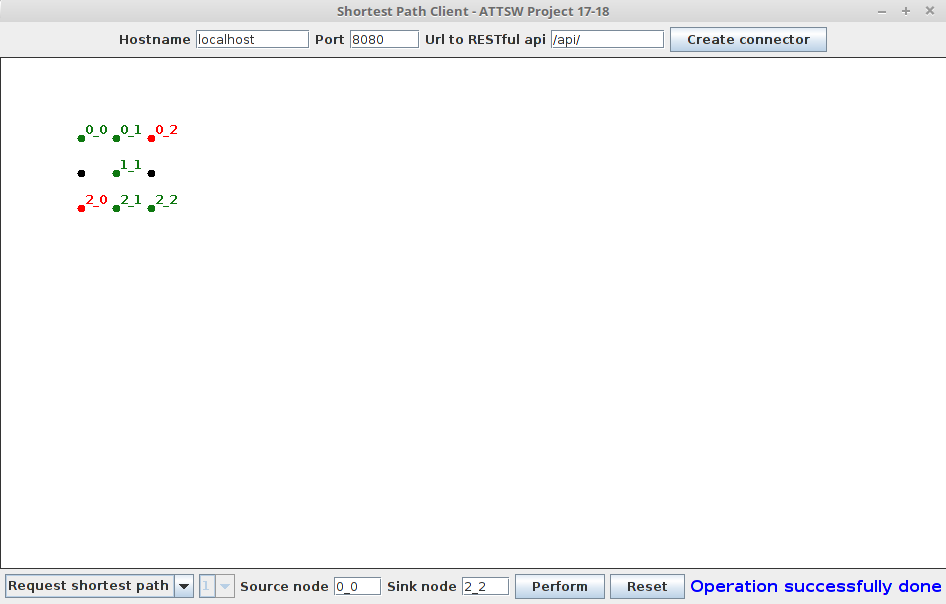
\includegraphics[width=0.7\linewidth]{Chapters/4}
	\caption[Interfaccia utente]{Richiedi il cammino minimo nella griglia 1 da 0,0 a 2,2}
	\label{fig:4}
\end{figure}

 \subsubsection{Implementazione dell'interfaccia}
 L'interfaccia fa uso del framework Swing. Essa \`e gestita da una classe GUI che ha al suo interno un'istanza di JFrame, una classe di Swing che rappresenta una finestra come comunemente intesa dall'utente. Come visto in precedenza, il frame \`e diviso in tre sezioni:
 \begin{itemize}
 	\item NORTH
 	\item CENTER
 	\item SOUTH
 \end{itemize}
A ciascuna di questa sezione corrisponde un JPanel. JPanel \`e una classe di Swing che funziona come container di componenti come pulsanti, barre di inserimento testuale, men\`u, ecc. La classe JPanel pu\`o essere estesa col fine di riscrivere il suo metodo \emph{paintComponent(Graphics g)}, il metodo delegato al disegno del container. Questo \`e quanto avviene per il JPanel corrispondente al centro della finestra; infatti quest'ultimo \`e un'istanza della classe GUIpanel e rappresenta il punto centrale di tutta l'interfaccia grafica realizzata.\\*
Un GUIpanel \`e un oggetto che ha al suo interno una matrice di punti indicizzati (ciascun punto \`e istanza della classe Point del medesimo framework) che possono essere creati e disegnati con differenti colori. Questa struttura si adatta al nostro sistema in quanto per visualizzare una griglia, oppure un cammino al suo interno, \`e sufficiente colorare i punti che fanno parte della griglia rispettivamente di colore rosso e di colore verde. I punti che non fanno parte della griglia e non sono indicizzati dalla matrice ricevuta dal server verranno disegnati come punti \emph{hidden} ossia dello stesso colore dello sfondo del container, cosicch\`e possano apparire all'utente come nascosti. Infine, i nodi indicizzati dalla matrice ricevuta dal server che non fanno parte della griglia, sono visualizzati come punti di colore nero.
\chapter{Problemi incontrati}
In questo capitolo parleremo dei problemi che abbiamo incontrato sia durante la stesura del codice che durante l'utilizzo delle tecniche oggetto di questo corso.
\section{Integration test su Mac}
Abbiamo avuto un problema relativo all'esecuzione degli Integration Test dell'interfaccia grafica del client su Mac OS X. Il problema \`e stato risolto includendo nel POM un modulo della libreria AssertJ che era richiesto a run-time dal sistema Mac. Per essere poi sicuri che successive modifiche continuassero a non creare problemi su Mac OS, ne abbiamo abilitato la relativa build su travis grazie al meccanismo delle build \emph{matrix}.
\section{Build Mac del Server su Travis}
Come riportato nella documentazione di Travis, quest'ultimo non supporta l'utilizzo di Docker sulle macchine remote quando impostate per utilizzare Mac OS; pertanto siamo stati costretti a disabilitare la build su Mac per quanto riguarda il server.
\section{End to end test}
Per realizzare gli end to end test abbiamo scritto un Junit test case che utilizzasse un server non mockato. Tuttavia questa particolare circostanza impone che prima del lancio del test venga eseguito il server in locale, cosa non implementabile in automatico su Travis. Per risolvere questa problematica abbiamo escluso la classe riguardante gli end to end test dalla build di maven, ma l'abbiamo lasciata a disposizione per il suo lancio direttamente da eclipse. Al fine di verificare che gli end to end test passassero anche quando l'applicazione Server non risiede esclusivamente sulla stessa macchina locale in cui si lancia il Client (localhost) abbiamo eseguito il deploy dell'applicazione su heroku (all'indirizzo \url{http://attsw-server.herokuapp.com}) in modo tale da poter inserire questo URL negli end to end test al posto del semplice localhost.
\section{Deployment su heroku}
Heroku non supporta nativamente l'utilizzo di un database anche se lanciato in un container Docker, pertanto abbiamo dovuto creare un ramo sul Server chiamato deploy-heroku, nel quale si utilizza una versione in-memory del database Mongo, supportata da una libreria specifica di Spring Boot. Pertanto \`e proprio questo il ramo che viene "pushato" sulla repository git remota di heroku.
\section{Utilizzo di due differenti database}
Abbiamo provato anche ad integrare un database MySQL all'interno del Server, tuttavia in corso d'opera sono sorti numerosi problemi le cui soluzioni avevano complicato troppo la struttura delle classi. I principali problemi incontrati sono stati:
\begin{itemize}
	\item Incongruenza di tipi: il tipo java intero viene mappato su un database MySQL come un long a 64 bit, mentre non esiste il tipo di dato matrice. Questo fatto ci aveva costretto a creare una seconda classe, compatibile con MySQL, che rappresentasse un'istanza di una griglia all'interno del database MySQL. 
	\item Differenti repository Spring: l'interfaccia IGridService vede esclusivamente DatabaseGrid, oggetti direttamente mappati all'interno del database Mongo tramite l'interfaccia nativa IMongoRepository. Questa interfaccia ha un suo equivalente per i database MySQL (CrudRepository) ma l'utilizzo dell'una e dell'altra interfaccia (IMongoRepository, CrudRepository) per le operazioni con il database aveva notevolmente complicato la struttura di IGridService, aggiungendovi una dipendenza esplicita da un'interfaccia \emph{Implementor}, da noi realizzata, la quale astraeva IMongoRepository e CrudRepository. 
	\item Testing del database: non siamo riusciti a testare le operazioni sul database quando effettuate su MySQL, infatti, sebbene a run-time gli oggetti venivano correttamente scritti sul database e letti dal database, durante i test le operazioni di scrittura mediante repository non producevano alcuna istanza all'interno del database. L'unica soluzione che siamo riusciti a trovare \`e stata quella di sostituire l'utilizzo della repository MySQL con l'utilizzo diretto di una query sul database; soluzione giudicata come fortemente sbagliata in quanto non utilizzava gli strumenti di Spring Boot.
\end{itemize} 
Per risolvere questi problemi abbiamo fatto un refactoring completo del codice su una nuova repository git. Approfittando di ci\`o abbiamo ripulito non solamente il codice dall'uso di MySQL, ma abbiamo avuto la possiblit\'a di realizzare meglio, grazie all'esperienza maturata in precedenza, anche le altre funzioni gi\'a realizzate sulla vecchia repository.
\section{Mutation testing con PitClipse}
Per effettuare mutation testing sugli unit-test abbiamo utilizzato il framework PitClipse, tuttavia quest'ultimo quando genera i mutanti del SUT, lo fa mutando anche classi che non fanno parte del SUT propriamente inteso per gli unit test. Questo fatto ha fatto si che esistessero mutanti sopravvissuti nei report di PitClipse, ma tutti i mutanti sopravvissuti sono mutanti di classi che non sono \emph{under-test} nel test case in questione.
\section{Testing dell'interfaccia grafica}
Per verificare che quando doveva essere disegnato un punto nel pannello centrale del Client (GUIpanel), questo venisse effettivamente disegnato, abbiamo voluto verificare che venisse chiamato il metodo fillOval coi giusti argomenti su un oggetto Graphics. Mockito tuttavia permette di effettuare asserzioni sull'invocazione di un metodo solo su oggetti mockati o oggetti spiati. A run-time, l'oggetto Graphics usato da un JPanel per disegnare il proprio contenuto, \`e istanza di una particolare sottoclasse final di Graphics, quindi quest'ultimo non pu\`o essere n\'e mockato n\'e spiato. Per risolvere questa problematica abbiamo creato una classe Wrapper di Graphics che estende Graphics, spiato un'istanza di quest'ultima, e nei test abbiamo invocato il metodo paintComponent(Graphics) (metodo delegato al disegno del pannello) passandovi l'istanza spiata. In questo modo abbiamo potuto verificare che venissero invocati correttamente i metodi fillOval all'interno della classe GUIpanel.








%--------------------------------------------------------------
\end{document}
%--------------------------------------------------------------